
%% forked from https://gits-15.sys.kth.se/giampi/kthlatex kthlatex-0.2rc4 on 2020-02-13
%% expanded upon by Gerald Q. Maguire Jr.
%% This template has been adapted by Anders Sjögren to the University
%% Engineering Program in Computer Science at KTH ICT. Adaptation is the
%% translation of English headings into Swedish as the addition of Swedish

\documentclass[final, english, biblatex]{kththesis}
%\documentclass[english, biblatex]{kththesis}
\usepackage[utf8]{inputenc}

%% Conventions for todo notes:
\newcommand*{\generalExpl}[1]{\todo[inline]{#1}}                

% Language specific information (currently in English or Swedish)
\newcommand*{\engExpl}[1]{\todo[inline, backgroundcolor=kth-lightgreen40]{#1}} %% \engExpl{English descriptions about formatting}
\newcommand*{\sweExpl}[1]{\todo[inline, backgroundcolor=kth-lightblue40]{#1}}  %% % \sweExpl{Text på svenska}

% warnings
\newcommand*{\warningExpl}[1]{\todo[inline, backgroundcolor=kth-lightred40]{#1}} %% \warningExpl{warnings}

% todo
\usepackage{xcolor}

\newcommand*{\ierror}[1]{\todo[inline, backgroundcolor=red!40]{#1}}
\newcommand*{\merror}[1]{\todo[backgroundcolor=red!40]{#1}}

\newcommand*{\iwarning}[1]{\todo[inline, backgroundcolor=yellow!40]{#1}}
\newcommand*{\mwarning}[1]{\todo[backgroundcolor=yellow!40]{#1}}

\newcommand*{\itodo}[1]{\todo[inline, backgroundcolor=blue!40]{#1}}
\newcommand*{\mtodo}[1]{\todo[backgroundcolor=blue!40]{#1}}

\newcommand*{\deadline}[1]{\todo[inline, backgroundcolor=purple!40]{Deadline: #1}}

% Uncomment to hide specific comments, to hide **all** ToDos add `final` to
% document class
% \renewcommand\warningExpl[1]{}
% \renewcommand\generalExpl[1]{}
% \renewcommand\engExpl[1]{}
% For example uncommenting the following line hides the Swedish language explanations

\renewcommand\sweExpl[1]{}


\usepackage[language=english,style=ieee,citestyle=numeric-comp,sorting=none,backend=biber]{biblatex}
\addbibresource{references.bib}

% include a variety of packages that are useful
\input{lib/includes}
\input{lib/kthcolors}

%\glsdisablehyper
%\makeglossaries
%\makenoidxglossaries
%%%% Local Variables:
%%% mode: latex
%%% TeX-master: t
%%% End:
% The following command is used with glossaries-extra
\setabbreviationstyle[acronym]{long-short}
% The form of the entries in this file is \newacronym{label}{acronym}{phrase}
%                                      or \newacronym[options]{label}{acronym}{phrase}
% see "User Manual for glossaries.sty" for the  details about the options, one example is shown below
% note the specification of the long form plural in the line below
\newacronym[longplural={Debugging Information Entities}]{DIE}{DIE}{Debugging Information Entity}
%
% The following example also uses options
\newacronym[shortplural={OSes}, firstplural={operating systems (OSes)}]{OS}{OS}{operating system}

\newacronym{KTH}{KTH}{KTH Royal Institute of Technology}

\newacronym{LIF}{LIF}{Leaky Integrate-and-Fire}
\newacronym{QIF}{QIF}{Quadratic Integrate-and-Fire}
\newacronym[shortplural={SGs}, longplural={Surrogate Gradients}]{SG}{SG}{Surrogate Gradient}
\newacronym{AdEx}{AdEx}{Adaptive Exponential Integrate-and-Fire}
\newacronym{HH}{HH}{Hodgkin-Huxley}
\newacronym{SPN}{SPN}{Striatal Projection Neuron}
\newacronym{EA}{EA}{Evolutionary Algorithm}
\newacronym{ML}{ML}{Machine Learning}
\newacronym{NN}{NN}{Neural Network}
\newacronym{ANN}{ANN}{Artificial Neural Network}
\newacronym{CNN}{CNN}{Convolutional Neural Network}
\newacronym{RNN}{RNN}{Recurrent Neural Network}
\newacronym{SNN}{SNN}{Spiking Neural Network}
\newacronym{ISI}{ISI}{Inter-Spike Interval}
\newacronym{MSE}{MSE}{Mean Squared Error}
\newacronym{MAE}{MAE}{Mean Absolute Error}
\newacronym{AD}{AD}{Automatic Differentiation}
\newacronym{BP}{BP}{Backpropagation}
\newacronym{BPTT}{BPTT}{Backpropagation Through Time}
\newacronym{HP}{HP}{Hyperparameter}

\newacronym{DTW}{DTW}{Dynamic Time Warping}
\newacronym{SDTW}{SDTW}{Soft Dynamic Time Warping}

\newacronym{JIT}{JIT}{Just-In-Time Compilation}
\newacronym{HPC}{HPC}{High-Performance Computing}
\newacronym{JVP}{JVP}{Jacobian-Vector Product}
\newacronym{VJP}{VJP}{Vector-Jacobian Product}

                %load the acronyms file

\input{lib/defines}  % load some additional definitions to make writing more consistent

% The following is needed in conjunction with generating the DiVA data with abstracts and keywords using the scontents package and a modified listings environment
%\usepackage{listings}   %  already included
\ExplSyntaxOn
\newcommand\typestoredx[2]{\expandafter\__scontents_typestored_internal:nn\expandafter{#1} {#2}}
\ExplSyntaxOff
\makeatletter
\let\verbatimsc\@undefined
\let\endverbatimsc\@undefined
\lst@AddToHook{Init}{\hyphenpenalty=50\relax}
\makeatother

\lstnewenvironment{verbatimsc}
    {
    \lstset{%
        basicstyle=\ttfamily\tiny,
        backgroundcolor=\color{white},
        %basicstyle=\tiny,
        %columns=fullflexible,
        columns=[l]fixed,
        language=[LaTeX]TeX,
        %numbers=left,
        %numberstyle=\tiny\color{gray},
        keywordstyle=\color{red},
        breaklines=true,                 % sets automatic line breaking
        breakatwhitespace=true,          % sets if automatic breaks should only happen at whitespace
        %keepspaces=false,
        breakindent=0em,
        %fancyvrb=true,
        frame=none,                     % turn off any box
        postbreak={}                    % turn off any hook arrow for continuation lines
    }
}{}

%% Add some more keyowrds to bring out the structure more
\lstdefinestyle{[LaTeX]TeX}{
morekeywords={begin, todo, textbf, textit, texttt}
}

%% definition of new command for bytefield package
\newcommand{\colorbitbox}[3]{%
	\rlap{\bitbox{#2}{\color{#1}\rule{\width}{\height}}}%
	\bitbox{#2}{#3}}

% define a left aligned table cell that is ragged right
\newcolumntype{L}[1]{>{\raggedright\let\newline\\\arraybackslash\hspace{0pt}}p{#1}}

\usepackage[plainpages=false]{hyperref}
\usepackage[all]{hypcap}	%% prevents an issue related to hyperref and caption linking

%% Acronyms
% note that nonumberlist - removes the cross references to the pages where the acronym appears
% note that super will set the descriptions text aligned
% note that nomain - does not produce a main glossary, thus only acronyms will be in the glossary
% note that nopostdot - will prevent there being a period at the end of each entry
\usepackage[acronym, style=super, section=section, nonumberlist, nomain, nopostdot]{glossaries}
\setlength{\glsdescwidth}{0.75\textwidth}
\usepackage[automake]{glossaries-extra}

\input{lib/includes-after-hyperref}

%\glsdisablehyper
\makeglossaries
%\makenoidxglossaries
%%% Local Variables:
%%% mode: latex
%%% TeX-master: t
%%% End:
% The following command is used with glossaries-extra
\setabbreviationstyle[acronym]{long-short}
% The form of the entries in this file is \newacronym{label}{acronym}{phrase}
%                                      or \newacronym[options]{label}{acronym}{phrase}
% see "User Manual for glossaries.sty" for the  details about the options, one example is shown below
% note the specification of the long form plural in the line below
\newacronym[longplural={Debugging Information Entities}]{DIE}{DIE}{Debugging Information Entity}
%
% The following example also uses options
\newacronym[shortplural={OSes}, firstplural={operating systems (OSes)}]{OS}{OS}{operating system}

\newacronym{KTH}{KTH}{KTH Royal Institute of Technology}

\newacronym{LIF}{LIF}{Leaky Integrate-and-Fire}
\newacronym{QIF}{QIF}{Quadratic Integrate-and-Fire}
\newacronym[shortplural={SGs}, longplural={Surrogate Gradients}]{SG}{SG}{Surrogate Gradient}
\newacronym{AdEx}{AdEx}{Adaptive Exponential Integrate-and-Fire}
\newacronym{HH}{HH}{Hodgkin-Huxley}
\newacronym{SPN}{SPN}{Striatal Projection Neuron}
\newacronym{EA}{EA}{Evolutionary Algorithm}
\newacronym{ML}{ML}{Machine Learning}
\newacronym{NN}{NN}{Neural Network}
\newacronym{ANN}{ANN}{Artificial Neural Network}
\newacronym{CNN}{CNN}{Convolutional Neural Network}
\newacronym{RNN}{RNN}{Recurrent Neural Network}
\newacronym{SNN}{SNN}{Spiking Neural Network}
\newacronym{ISI}{ISI}{Inter-Spike Interval}
\newacronym{MSE}{MSE}{Mean Squared Error}
\newacronym{MAE}{MAE}{Mean Absolute Error}
\newacronym{AD}{AD}{Automatic Differentiation}
\newacronym{BP}{BP}{Backpropagation}
\newacronym{BPTT}{BPTT}{Backpropagation Through Time}
\newacronym{HP}{HP}{Hyperparameter}

\newacronym{DTW}{DTW}{Dynamic Time Warping}
\newacronym{SDTW}{SDTW}{Soft Dynamic Time Warping}

\newacronym{JIT}{JIT}{Just-In-Time Compilation}
\newacronym{HPC}{HPC}{High-Performance Computing}
\newacronym{JVP}{JVP}{Jacobian-Vector Product}
\newacronym{VJP}{VJP}{Vector-Jacobian Product}

                %load the acronyms file

% insert the configuration information with author(s), examiner, supervisor(s), ...
%% Information for inside title page


\authorsLastname{Mayer}
\authorsFirstname{Paul}
\email{pmayer@kth.se}
\kthid{u100001} % TODO!!!!
% As per email from KTH Biblioteket on 2021-06-28 students cannot have an OrCiD reported for their degree project
\authorsSchool{\schoolAcronym{EECS}}
%If the student is not in Stockholm, Sweden, add that information here
% This information will be used when generating the acknowledgements signature.
%\authorCity{A City}
%\authorCountry{A Country}
% pass into \authorCityCountryDate{} the month and year for the acknowledgment
% If there is a second author and place, the month, and year are the same, the specify the month and year for the first author:
\authorCityCountryDate{\MONTH\enspace\the\year}
% if there is a second author and the place is different, then say:
%\authorCityCountryDate{}

\supervisorAsLastname{Kozlov}
\supervisorAsFirstname{Alexander}
\supervisorAsEmail{akozlov@kth.se}
% If the supervisor is from within KTH add their KTHID, School and Department info

\supervisorAsKTHID{} % TODO!!!!
\supervisorAsSchool{\schoolAcronym{EECS}}
\supervisorAsDepartment{Computer Science} % TODO: Check this!

\examinersLastname{Fransén}
\examinersFirstname{Erik}
\examinersEmail{erikf@kth.se}
% If the examiner is from within KTH add their KTHID, School and Department info
\examinersKTHID{} % TODO!!!!
\examinersSchool{\schoolAcronym{EECS}}
\examinersDepartment{Computer Science} % TODO: check this!!!

\date{\today}

\courseCycle{2}
\courseCode{DA231X}
\courseCredits{30.0}

\programcode{TCSCM}
\degreeName{Master's Programme, Computer Science, 120 credits}
\subjectArea{Computer Science}

%%%%% for DiVA's National Subject Category information
%%% Enter one or more 3 or 5 digit codes
%%% See https://www.scb.se/contentassets/3a12f556522d4bdc887c4838a37c7ec7/standard-for-svensk-indelning--av-forskningsamnen-2011-uppdaterad-aug-2016.pdf
%%% See https://www.scb.se/contentassets/10054f2ef27c437884e8cde0d38b9cc4/oversattningsnyckel-forskningsamnen.pdf
%%%%
%%%% Some examples of these codes are shown below:
% 102 Data- och informationsvetenskap (Datateknik)    Computer and Information Sciences
% 10201 Datavetenskap (datalogi) Computer Sciences 
% 10202 Systemvetenskap, informationssystem och informatik (samhällsvetenskaplig inriktning under 50804)
% Information Systems (Social aspects to be 50804)
% 10203 Bioinformatik (beräkningsbiologi) (tillämpningar under 10610)
% Bioinformatics (Computational Biology) (applications to be 10610)
% 10204 Människa-datorinteraktion (interaktionsdesign) (Samhällsvetenskapliga aspekter under 50803) Human Computer Interaction (Social aspects to be 50803)
% 10205 Programvaruteknik Software Engineering
% 10206 Datorteknik Computer Engineering
% 10207 Datorseende och robotik (autonoma system) Computer Vision and Robotics (Autonomous Systems)
% 10208 Språkteknologi (språkvetenskaplig databehandling) Language Technology (Computational Linguistics)
% 10209 Medieteknik Media and Communication Technology
% 10299 Annan data- och informationsvetenskap Other Computer and Information Science
%%%
% 202 Elektroteknik och elektronik Electrical Engineering, Electronic Engineering, Information Engineering
% 20201 Robotteknik och automation Robotics
% 20202 Reglerteknik Control Engineering
% 20203 Kommunikationssystem Communication Systems
% 20204 Telekommunikation Telecommunications
% 20205 Signalbehandling Signal Processing
% 20206 Datorsystem Computer Systems
% 20207 Inbäddad systemteknik Embedded Systems
% 20299 Annan elektroteknik och elektronik Other Electrical Engineering, Electronic Engineering, Information Engineering
%% Example for a thesis in Computer Science and Computer Systems
\nationalsubjectcategories{10201, 10203}




\title{Surrogate Gradients for Gradient-Based Parameter Estimation in Simplified Neuron Models}
\subtitle{THESIS SUB TOPIC}

% give the alternative title - i.e., if the thesis is in English, then give a Swedish title
\alttitle{Detta är den svenska översättningen av titeln}
\altsubtitle{Detta är den svenska översättningen av undertiteln}
% alternative, if the thesis is in Swedish, then give an English title
%\alttitle{This is the English translation of the title}
%\altsubtitle{This is the English translation of the subtitle}

% Enter the English and Swedish keywords here for use in the PDF meta data _and_ for later use
% following the respective abstract.
% Try to put the words in the same order in both languages to facilitate matching. For example:
\EnglishKeywords{Automatic Gradient Descent, Integrate-and-Fire Model, Simplified Neuron Model, Surrogate Gradients, Parameter Estimation}
\SwedishKeywords{TODO KEYWORDS SWEDSISH}
\GermanKeywords{TODO KEYWORDS GERMAN}

%%%%% For the oral presentation
%% Add this information once your examiner has scheduled your oral presentation
\presentationDateAndTimeISO{2022-03-15 13:00}
\presentationLanguage{eng}
\presentationRoom{via Zoom https://kth-se.zoom.us/j/ddddddddddd}
\presentationAddress{Isafjordsgatan 22 (Kistagången 16)}
\presentationCity{Stockholm}

% When there are multiple opponents, separate their names with '\&'
% Opponent's information
\opponentsNames{A. B. Normal \& A. X. E. Normalè}

% Once a thesis is approved by the examiner, add the TRITA number
% The TRITA number for a thesis consists of two parts a series (unique to each school)
% and the number in the series which is formatted as the year followed by a colon and
% then a unique series number for the thesis - starting with 1 each year.
\trita{TRITA-EECS-EX}{2022:00}

% Put the title, author, and keyword information into the PDF meta information
\input{lib/pdf_related_includes}


% the custom colors and the commands are defined in defines.tex    
\hypersetup{
	colorlinks  = true,
	breaklinks  = true,
	linkcolor   = \linkscolor,
	urlcolor    = \urlscolor,
	citecolor   = \refscolor,
	anchorcolor = black
}

\ifnomenclature
% The following lines make the page numbers and equations hyperlinks in the Nomenclature list
\renewcommand*{\pagedeclaration}[1]{\unskip, \dotfill\hyperlink{page.#1}{page\nobreakspace#1}}
% The following does not work correctly, as the name of the cross-reference is incorrect
%\renewcommand*{\eqdeclaration}[1]{, see equation\nobreakspace(\hyperlink{equation.#1}{#1})}

% You can also change the page heading for the nomenclature
\renewcommand{\nomname}{List of Symbols Used}

% You can even add customization text before the list
\renewcommand{\nompreamble}{The following symbols will be later used within the body of the thesis.}
\makenomenclature
\fi

%
% The commands below are to configure JSON listings
% 
% format for JSON listings
\colorlet{punct}{red!60!black}
\definecolor{delim}{RGB}{20,105,176}
\definecolor{numb}{RGB}{106, 109, 32}
\definecolor{string}{RGB}{0, 0, 0}

\lstdefinelanguage{json}{
    numbers=none,
    numberstyle=\small,
    frame=none,
    rulecolor=\color{black},
    showspaces=false,
    showtabs=false,
    breaklines=true,
    postbreak=\raisebox{0ex}[0ex][0ex]{\ensuremath{\color{gray}\hookrightarrow\space}},
    breakatwhitespace=true,
    basicstyle=\ttfamily\small,
    extendedchars=false,
    upquote=true,
    morestring=[b]",
    stringstyle=\color{string},
    literate=
     *{0}{{{\color{numb}0}}}{1}
      {1}{{{\color{numb}1}}}{1}
      {2}{{{\color{numb}2}}}{1}
      {3}{{{\color{numb}3}}}{1}
      {4}{{{\color{numb}4}}}{1}
      {5}{{{\color{numb}5}}}{1}
      {6}{{{\color{numb}6}}}{1}
      {7}{{{\color{numb}7}}}{1}
      {8}{{{\color{numb}8}}}{1}
      {9}{{{\color{numb}9}}}{1}
      {:}{{{\color{punct}{:}}}}{1}
      {,}{{{\color{punct}{,}}}}{1}
      {\{}{{{\color{delim}{\{}}}}{1}
      {\}}{{{\color{delim}{\}}}}}{1}
      {[}{{{\color{delim}{[}}}}{1}
      {]}{{{\color{delim}{]}}}}{1}
      {’}{{\char13}}1,
}

\lstdefinelanguage{XML}
{
  basicstyle=\ttfamily\color{blue}\bfseries\small,
  morestring=[b]",
  morestring=[s]{>}{<},
  morecomment=[s]{<?}{?>},
  stringstyle=\color{black},
  identifierstyle=\color{blue},
  keywordstyle=\color{cyan},
  breaklines=true,
  postbreak=\raisebox{0ex}[0ex][0ex]{\ensuremath{\color{gray}\hookrightarrow\space}},
  breakatwhitespace=true,
  morekeywords={xmlns,version,type}% list your attributes here
}

% In case you use both listings and lstlistings - this makes them both use the same counter
\makeatletter
\AtBeginDocument{\let\c@listing\c@lstlisting}
\makeatother
\usepackage{subfiles}

% To have Creative Commons (CC) license and logos use the doclicense package
% Note that the lowercase version of the license has to be used in the modifier
% i.e., one of by, by-nc, by-nd, by-nc-nd, by-sa, by-nc-sa, zero.
% For background see:
% https://www.kb.se/samverkan-och-utveckling/oppen-tillgang-och-bibsamkonsortiet/open-access-and-bibsam-consortium/open-access/creative-commons-faq-for-researchers.html
% https://kib.ki.se/en/publish-analyse/publish-your-article-open-access/open-licence-your-publication-cc
\begin{comment}
\usepackage[
    type={CC},
    %modifier={by-nc-nd},
    %version={4.0},
    modifier={by-nc},
    imagemodifier={-eu-88x31},  % to get Euro symbol rather than Dollar sign
    hyphenation={RaggedRight},
    version={4.0},
    %modifier={zero},
    %version={1.0},
]{doclicense}
\end{comment}

\begin{document}
%\selectlanguage{swedish}
%
\selectlanguage{english}

%%% Set the numbering for the title page to a numbering series not in the preface or body
\pagenumbering{alph}
\kthcover
\clearpage\thispagestyle{empty}\mbox{} % empty back of front cover
\titlepage

% If you do not want to have a bookinfo page, comment out the line saying \bookinfopage and add a \cleardoublepage
% If you want a bookinfo page: you will get a copyright notice, unless you have used the doclicense package in which case you will get a Creative Commons license. To include the doclicense package, uncomment the configuration of this package above and configure it with your choice of license.
\bookinfopage

% Frontmatter includes the abstracts and table-of-contents
\frontmatter

\cleardoublepage
\listoftodos

\cleardoublepage
\setcounter{page}{1}
\begin{abstract}
% The first abstract should be in the language of the thesis.
% Abstract fungerar på svenska också.
  \markboth{\abstractname}{}
\begin{scontents}[store-env=lang]
eng
\end{scontents}
%%% The contents of the abstract (between the begin and end of scontents) will be saved in LaTeX format
%%% and output on the page(s) at the end of the thesis with information for DiVA facilitating the correct
%%% entry of the meta data for your thesis.
%%% These page(s) will be removed before the thesis is inserted into DiVA.

\begin{scontents}[store-env=abstracts,print-env=true]
  \itodo{Abstract}
\end{scontents}

\subsection*{Keywords}
\begin{scontents}[store-env=keywords,print-env=true]
\InsertKeywords{english}
\end{scontents}
\end{abstract}

\cleardoublepage
\babelpolyLangStart{swedish}
\begin{abstract}
    \markboth{\abstractname}{}
\begin{scontents}[store-env=lang]
swe
\end{scontents}
\begin{scontents}[store-env=abstracts,print-env=true]
  \itodo{Swedish Abstract}
\end{scontents}
\subsection*{Nyckelord}
\begin{scontents}[store-env=keywords,print-env=true]
\InsertKeywords{swedish}
\end{scontents}
\end{abstract}
\babelpolyLangStop{swedish}

\cleardoublepage
\babelpolyLangStart{ngerman}
\begin{abstract}
    \markboth{\abstractname}{}
\begin{scontents}[store-env=lang]
ger
\end{scontents}
\begin{scontents}[store-env=abstracts,print-env=true]
  \itodo{Zusammenfassung}
\end{scontents}
\subsection*{Schlüsselwörter}
\begin{scontents}[store-env=keywords,print-env=true]
\InsertKeywords{german}
\end{scontents}
\end{abstract}
\babelpolyLangStop{ngerman}
\cleardoublepage

\section*{Acknowledgments}
\markboth{Acknowledgments}{}
  \itodo{Acknowledgments}
\acknowlegmentssignature

\fancypagestyle{plain}{}
\renewcommand{\chaptermark}[1]{ \markboth{#1}{}} 
\tableofcontents
  \markboth{\contentsname}{}

\cleardoublepage
\listoffigures

\cleardoublepage

\listoftables
\cleardoublepage
\lstlistoflistings\engExpl{If you have listings in your thesis. If not, then remove this preface page.}
\cleardoublepage
% Align the text expansion of the glossary entries
\newglossarystyle{mylong}{%
  \setglossarystyle{long}%
  \renewenvironment{theglossary}%
     {\begin{longtable}[l]{@{}p{\dimexpr 2cm-\tabcolsep}p{0.8\hsize}}}% <-- change the value here
     {\end{longtable}}%
 }
%\glsaddall
%\printglossaries[type=\acronymtype, title={List of acronyms}]
\printglossary[style=mylong, type=\acronymtype, title={List of acronyms and abbreviations}]
%\printglossary[type=\acronymtype, title={List of acronyms and abbreviations}]

%\printnoidxglossary[style=mylong, title={List of acronyms and abbreviations}]
\engExpl{The list of acronyms and abbreviations should be in alphabetical order based on the spelling of the acronym or abbreviation.
}

% if the nomenclature option was specified, then include the nomenclature page(s)
\ifnomenclature
    \cleardoublepage
    % Output the nomenclature list
    \printnomenclature
\fi

%% The following label is essential to know the page number of the last page of the preface
%% It is used to computer the data for the "For DIVA" pages
\label{pg:lastPageofPreface}
% Mainmatter is where the actual contents of the thesis goes
\mainmatter
\glsresetall
\renewcommand{\chaptermark}[1]{\markboth{#1}{}}
\selectlanguage{english}

\itodo{Check custom\_configuration.tex!!!}
\itodo{Change subtitle}
\itodo{Change opponent}
\itodo{Swedish title}
\itodo{Swedish subtitle}
\itodo{Keywords}
\itodo{Keywords swedish}
\itodo{Keywords german}


% End of Abstract
% ----------------------------------------------------------------------------------------------
%  Content


\chapter{Introduction}
\label{ch:introduction}
\deadline{May 31st, 5-10 pages}

\itodo{Structure of this chapter can change, should more or less reflect the structure of whole thesis}

\section{Background}
\section{Problem}
\section{Purpose}
\section{Goals}
\section{Method}
\section{Limitations}
\section{Overview}

\cleardoublepage
\chapter{Background}
\label{ch:background}
\deadline{Feb 28th, BG + RL 10-20 pages}
\itodo{Write introduction paragraph of background section so that chapter doesn't start with section title}

\section{Neuron Models}
Large-scale brain models are limited in size mostly by computational feasibility.
Detailed bio-physical models like the \gls{HH}-model can precisely predict membrane behaviour of a vast variety of neuron types.
However, they require huge computational resources to estimate the required parameters to fit the models to experimental data.
Simplified Neuron Models models overcome this challenge, capturing most of the sophisticated neuron behaviour with only a fraction of the computational cost, enabling large-scale simulations \cite{Gerstner2014}.
The \gls{AdEx} model \cite{Naud2008} provides a particularly interesting balance --- it reproduces a variety of firing patterns but drastically reduces the number of necessary parameters of the model.
This makes it a favourable model for large-scale neuron simulations \cite{Tesler2024}\mwarning{Should there be that many citations here? Mostly Textbook citations, make sure of that}.

The \gls{AdEx} model improves the simpler \gls{LIF} model in two ways:
first, it introduces exponential behaviour when initialising the spike.
Second, the model allows for adaptation, meaning it can change spiking frequencies or post-spike refractoriness based on their firing history.
It is defined by the equations given in \cite{Brette2005, Naud2008}:
\begin{align}
  C \frac{dV}{dt} &= -g_L (V - E_L) + g_L \Delta_T \exp(\frac{V - V_T}{\Delta_T}) + I - w,\label{eq:adex1}\\
  \tau_w \frac{dw}{dt} &= a(V - E_L) - w,\label{eq:adex2}
\end{align}
with the following reset condition:
\begin{align}
  \text{if } V > 0 \text{ mV}\; \text{ then} &= \begin{cases}
    V \rightarrow V_r,\\
    w \rightarrow w_r = w + b.
  \end{cases}\label{eq:adex3}
\end{align}

It describes the membrane potential over time $V(t)$ given an injected current $I(t)$.
Equation (\ref{eq:adex1}) describes the change of potential.
$C$ is the membrane capacitance, $g_L$ the leak conductance and $E_L$ the effective resting potential.
We can understand $-g_L (V - E_L)$ as the leak current that slowly pulls the membrane potential towards its resting potential.
$g_L \Delta_T \exp(\frac{V - V_T}{\Delta_T})$ models the depolarisation initialised by the fast reacting sodium channels using an exponential function,
modelled using a driving force based on an effective threshold potential $V_T$ and a slope factor $\Delta_T$.
$I$ is the injected current, and $w$ is the adaptation current, which is described in equation \ref{eq:adex2}.

The adaptation mechanism is controlled via an adaptation current which opposes depolarisation.
Unlike the fast membrane behaviour, this current is related to the time constant $\tau_w$, which controls the decay time.
It is controlled by $a$ (sub-threshold adaptation) as well as $b$ (spike-triggered adaptation).

Even though the number of parameters is significantly reduced compared to bio-physical \gls{HH}-type models, it still requires parameter fitting --- especially because some parameters (e.g. $a$, $b$ or $\tau_w$) do not have direct physiological counterparts (like $C$ or $g_L$).
For AdEx to perform as an effective tool, efficient methods for parameter optimizations are essential.

\section{Parameter Tuning for Neuron Models}
A central challenge in neuroscience has been to 'identify the parameters of detailed biophysical models, such that they match physiological measurements at scale' \cite{Deistler2025} in reasonable simulation runtimes.
The zoo of optimisation techniques is large, spanning from evolutionary algorithms \cite{VanGeit2008} to gradient descent \cite{Jones2024}, however, deciding which algorithm to use may often depend on the underlying properties of the model.
\texttt{Jaxley} \cite{Deistler2025}, a newly developed framework, uses automatic differentiation to quickly fit parameters of sophisticated biophysical models to experimental data and perform large-scale neuron simulations.
Specifically, \texttt{Jaxley} allows to simulate multi-compartment models with complex structures (dendrites, axons), cable theory equations and \gls{HH}-type ion channels.
To perform parameter optimisation, \texttt{Jaxley} uses automatic differentiation (via \texttt{Jax}).
It shows very promising results, matching or outperforming other state-of-the-art (e.g. genetic algorithms) in performance for small and large neuron models respectively.
However, as previously stated, in many circumstances it still remains unfeasible to use \gls{HH}-type models for large-scale simulations.
\texttt{Jaxley} fails to support simplified models to perform parameter tuning.
The fundamental limitation is that simplified models are not by default automatically differentiable.
This is a result of the reset condition in equation~\ref{eq:adex3}.
Addressing this issues requires special treatment: surrogate gradients.
\mtodo{Introduce Nelder-Mead (or is this related work?)}

\section{Surrogate Gradients}
\gls{SG} were developed to adapt spiking neurons (usually using \gls{LIF} neuron models) for training, primarily on classification tasks.
To fit these models to real data, the typical forward pass - backward pass strategy needed to be enabled.
Because \gls{LIF}-type models have a discontinuous derivatives (see reset in equation~\ref{eq:adex3}), automatic differentiation cannot be performed without adjustments.
To overcome this issue, prior work replaced the discontinues (heavyside-) functions derivative with a (e.g. sigmoid) surrogate, but only for the backward pass \cite{Neftci2019}.
For training weights in \gls{SNN}, this performed sufficiently well.
\mwarning{This should be extended, there is a lot more to say, e.g. what loss functions do they use?}

\section{Optimization Problems/Loss Functions}
\itodo{Loss function Background}

\section{Summary}
\itodo{Background summary}

\cleardoublepage
\chapter{Related Work}\label{ch:relwork}
\deadline{Feb 28th}

\mwarning{Should this be it's own chapter, or should this be a section in the baground? I personally may prefer to keep it separate it's own chapter...}
Simplified Neuron Models historically were a necessity to deal with the fact that computing resources were too limited to perform large scale brain simulations with sophisticated ion-channel based models.
With the rise of cheap and widely available supercomputing, focus shifted back to more detailed \gls{HH}-type model.
In recent years however, interest in simplified models resurged, driven by mainly two reasons: researchers wanting to progress \gls{ANN} to use more detailed spiking neurons and computational neuroscientists getting closer to feasibly simulating whole mammal brains.

\section{Parameter Estimation for AdEx Model}
A neuron model has to replicate behaviour of a huge variety of neurons.
In simplified neuron models like \gls{AdEx}, some parameters lack a real (measurable) counterpart.
Therefore parameters have to be estimated using optimisation techniques.
Traditionally, a huge variety (from evolutionary strategies to particle swarm optimizations) of approaches were used \cite{VanGeit2008}.
A very recent paper uses grid search over a feature space, not gradients \cite{Guarino2025}.
Recently genetic algorithms, multi-state single-agent stochastic search (MSASS) or Teaching-Learning-Based Optimization (TLBO) have been used successfully to tune parameters for the \gls{AdEx} model to real voltage-clamp recordings \cite{Marin2020, Cruz2021}.
However, these approaches tend to use a lot of computational resources.

Hertag et al. \cite{Hertag2011} developed an analytical approximation to the AdEx model to speed up computations.
Using automatic differentiation could also address this issue.
Jones et al. \cite{Jones2024} and Deistler et al. \cite{Deistler2025} demonstrated that gradient-based methods can effectively parametrize HH-type models.
However, they require the inherently differentiable nature of HH-type models.
Simplified models require additional treatment to benefit from this technique.

\section{Parameter Learning using Surrogate Gradients in Spiking Neural Networks}
Previous work explored using surrogate gradients for training weights of \gls{SNN} in classification tasks \cite{Neftci2019, Gerum2021, Perez-Nieves2021}.
Gerum and Schilling \cite{Gerum2021} explored different surrogates (like sigmoid or esser function) to train a \gls{LIF} based \gls{NN} for image classification tasks.
The authors used \texttt{Keras} to perform automatic differentiation and backpropagation.
Perez-Nieves et al. \cite{Perez-Nieves2021} used a sigmoidal surrogate gradient in the backward pass to train a spiking NN in \texttt{PyTorch} to perform a variety of different classification tasks.
However, their work focuses on training network weights on task-based classification tasks.

Recent theoretical work \cite{Gygax2025} clarifies why surrogate gradients succeed despite approximating the true gradient.
But fitting biophysical parameters to experimental recordings poses a different challenge:
the loss function must quantify similarity between simulated and recorded spike trains.
Whether standard choices like mean squared error suffice --- 
or whether domain-specific alternatives are required --- 
remains unexplored.
This work investigates this question.
\itodo{Introduce Nelder-Mead? Latest Simplex Algorithms...}

\section{Benchmark Sets for Neuron Models}
Neuron models are highly specialised and are fit to very specific data.
Therefore it proves to be difficult to compare models systematically.
Jolivet et al. \cite{Jolivet2008} introduce a coincidence factor, which allows to evaluate neuron models.
We use this concept to evaluate the quality of our trained parameters.
\itodo{This has to be extended!}

\section{Loss Functions}
\itodo{Differentiable Loss functions, e.g. soft dynamic time warping or other.}

\section{Relevance}
\iwarning{This may not be it's own section and rather be a paragraph in each of the other sections, but it could also be a good idea to conclude it here.}

\cleardoublepage
\chapter{Methodology}
\label{ch:method}

This work introduces two contributions: firstly, we implement the \gls{AdEx} model within \texttt{Jaxley}, providing both standard and surrogate gradient variants.
The surrogate implementation can easily adopted to Jaxleys existing simplified models: \gls{LIF} and Izhikevich.
Secondly, we use \texttt{Jaxley} to perform gradient-based optimisation.
We investigate two\merror{update this to the correct amount} different loss functions:
\begin{itemize}
  \item \mwarning{What about absolute error}\gls{MSE}
  \item \itodo{Introduce dynamic time warping}
  \item Guarino et al. \cite{Guarino2025} feature-based loss function.
\end{itemize}
Using gradient-based optimisation requires a differentiable loss function.
Therefore we will introduce a gradient version of the feature-based loss function.

\section{Integration of Surrogate Gradients into Jaxley}
\texttt{Jaxley} is built on top of \texttt{JAX} and leverages its automatic differentiation capabilities for gradient-based parameter optimisation.
Neuron dynamics in \texttt{Jaxley} are defined through \texttt{Channel} classes, which specify three core methods: \texttt{update\_states()} for state variable evolution, \texttt{compute\_current()} for membrane current contributions, and \texttt{init\_state()} for initialisation of state variables.
During simulation, \texttt{JAX} traces these functions to construct a computational graph, enabling automatic gradient computation and backpropagation.

\subsection{The Differentiability Problem}
Simplified neuron models employ a discrete reset mechanism when the membrane potential crosses a threshold.
This reset is mathematically expressed using the Heavyside step function $H$:
\begin{equation}
    H(v - v_{\text{th}}) = \begin{cases} 1 & \text{if } v \geq v_{\text{th}} \\ 0 & \text{otherwise} \end{cases}
\end{equation}
The derivative of the Heavyside function is zero almost everywhere (and undefined at the threshold):
\begin{equation}
    \frac{\partial H}{\partial v} = 0 \quad \text{for } v \neq v_{\text{th}}
\end{equation}
This causes gradients to vanish during back-propagation through spike events, which prevents gradient-based optimisation from working.

\subsection{Surrogate Gradient Approach}
To overcome this limitation, we employ surrogate gradients \cite{Neftci2019}: the forward pass uses the original Heavyside function to maintain correct spike dynamics, while the backward pass substitutes the function with a surrogate.
This is implemented in \texttt{JAX} using \texttt{jax.custom\_vjp}, which allows defining custom vector-Jacobian products.

We implement three surrogate gradient functions, each providing different gradient characteristics:

\textbf{Sigmoid surrogate:}
\begin{equation}
    \frac{\partial \tilde{H}}{\partial x} = \beta \cdot \sigma(\beta x) \cdot (1 - \sigma(\beta x))
\end{equation}
where $\sigma$ is the sigmoid function and $\beta$ controls the steepness.

\textbf{Exponential surrogate:}
\begin{equation}
    \frac{\partial \tilde{H}}{\partial x} = \beta \cdot \exp(-\beta |x|)
\end{equation}

\textbf{SuperSpike surrogate} \cite{Zenke2018}:
\begin{equation}
    \frac{\partial \tilde{H}}{\partial x} = \frac{1}{(\beta |x| + 1)^2}
\end{equation}

All three surrogates are centred at the threshold ($x = v - v_{\text{th}}$).
The hyperparameter $\beta$ controls the sharpness: higher values produce steeper gradients at the threshold, while lower values spread the gradient over a wider voltage ranges.

\subsection{Implementation Details}
We reformulate the conditional reset from a discrete selection:
\begin{equation}
    v_{\text{new}} = \begin{cases} v_{\text{reset}} & \text{if spike} \\ v & \text{otherwise} \end{cases}
\end{equation}
to a continuous, differentiable form:
\begin{equation}
    v_{\text{new}} = s \cdot v_{\text{reset}} + (1 - s) \cdot v
\end{equation}
where $s = \tilde{H}(v - v_{\text{th}})$ is the surrogate spike indicator, to ensure differentiability through the reset mechanism.
This formulation allows gradients to flow through the reset operation.

This approach can easily be applied to the existing \gls{LIF} (\texttt{Fire\-Surrogate}) and Izhikevich models in \texttt{Jax\-ley},
not only to the newly implemented \gls{AdEx} model (\texttt{AdEx\-Surro\-gate}).

\section{AdEx Model Implementation}\label{sec:adex_impl}
We implement the \gls{AdEx} model as a \texttt{Jaxley} channel, following the formulation by Brette and Gerstner \cite{Brette2005} (see Equations~\ref{eq:adex1}--\ref{eq:adex3}).
Unlike \gls{HH}-type channels that contribute currents to a shared voltage solver, simplified models like \gls{AdEx} handle voltage integration directly within their \texttt{update\_states()} method.
We follow the implementation pattern of \cite{Deistler2025}.

\subsection{Numerical Integration}
The \gls{AdEx} model consists of two coupled differential equations requiring different numerical treatment:

\textbf{Adaptation current $w$:}
Equation~\ref{eq:adex2} is a linear dynamic system in $w$, allowing the use of exponential Euler integration.
It has the analytical solution
\begin{equation}
  w(t+\Delta t) = w(t) \cdot e^{-\Delta t / \tau_w} + a(V - E_L)(1 - e^{-\Delta t / \tau_w})
\end{equation}\label{eq:adaption-current-integration}
which gives increased numerical stability compared to e.g. forward euler methods.

\textbf{Membrane potential $V$:}
The exponential term in Equation~\ref{eq:adex1} makes this equation nonlinear, requiring forward Euler integration:
\begin{equation}
    V(t + \Delta t) = V(t) + \Delta t \cdot \frac{dV}{dt}
\end{equation}
To prevent numerical overflow from the exponential spike mechanism, we clamp the argument:
\begin{equation}
    \exp\left(\frac{V - V_T}{\Delta_T}\right) \rightarrow \exp\left(\min\left(\frac{V - V_T}{\Delta_T}, 10\right)\right)
\end{equation}

\subsection{Spike Detection and Reset}
After each integration step, we check for threshold crossing ($V > v_{\text{threshold}}$).
If the threshold is crossed, we apply the reset conditions from Equation~\ref{eq:adex3}.
For standard \texttt{LIF}, \texttt{AdEx} or \texttt{Izhikevich}, this uses \texttt{jax.lax.select()} for conditional assignment.
In the differentiable variants, we use the continuous formulation described in Section~\ref{sec:method} for both $V$ and $w$:
\begin{align}
    V_{\text{new}} &= s \cdot V_r + (1 - s) \cdot V, \\
    w_{\text{new}} &= s \cdot (w + b) + (1 - s) \cdot w,
\end{align}
where $s: V\rightarrow [0,1]$ is the surrogate of the heavyside function.

\subsection{Model Parameters}
Table~\ref{tab:adex_params} summarises the \gls{AdEx} parameters and their default values.
Parameters without direct physiological counterparts (e.g., $a$, $b$, $\tau_w$) are primary targets for optimisation.
\itodo{Welche Parameter haben eine biologischen Gegenspieler? Kann ich hier frei wählen, was ist warum wie eingeschränkt?}

\begin{table}[t]
\centering
\caption{\gls{AdEx} model parameters and default values.}
\label{tab:adex_params}
\begin{tabular}{llll}
\toprule
\textbf{Parameter} & \textbf{Symbol} & \textbf{Default} & \textbf{Unit} \\
\midrule
Membrane capacitance & $C$ & 200 & pF \\
Leak conductance & $g_L$ & 10 & nS \\
Leak reversal & $E_L$ & -70 & mV \\
Threshold potential & $V_T$ & -50 & mV \\
Slope factor & $\Delta_T$ & 2 & mV \\
Reset potential & $V_r$ & -58 & mV \\
Detection threshold & $v_{\text{threshold}}$ & 0 & mV \\
Adaptation time constant & $\tau_w$ & 30 & ms \\
Subthreshold adaptation & $a$ & 2 & nS \\
Spike-triggered adaptation & $b$ & 0 & pA \\
Stimulation current & $I$ & 500 & pA\\
\bottomrule
\end{tabular}
\end{table}

AdEx is defined using absolute capacitance ($pF$).
However, Jaxley is targeted at bio-physical HH-type simulations, and therefore works with cell morphology and gemoetries.
It therefore expects specific capacitance ($\mu F/cm^2$).
To circumvent this problem, we compute a fictitious cylindrical geometries whose surface area yields the desired total capacitance assuming jaxleys standard specific capacitance ($1 \mu F/cm^2$).
This scales injected currents to maintain correct dynamics.

\subsection{Implementation Verification}\label{sec:verification}
\begin{figure*}
  \begin{center}
    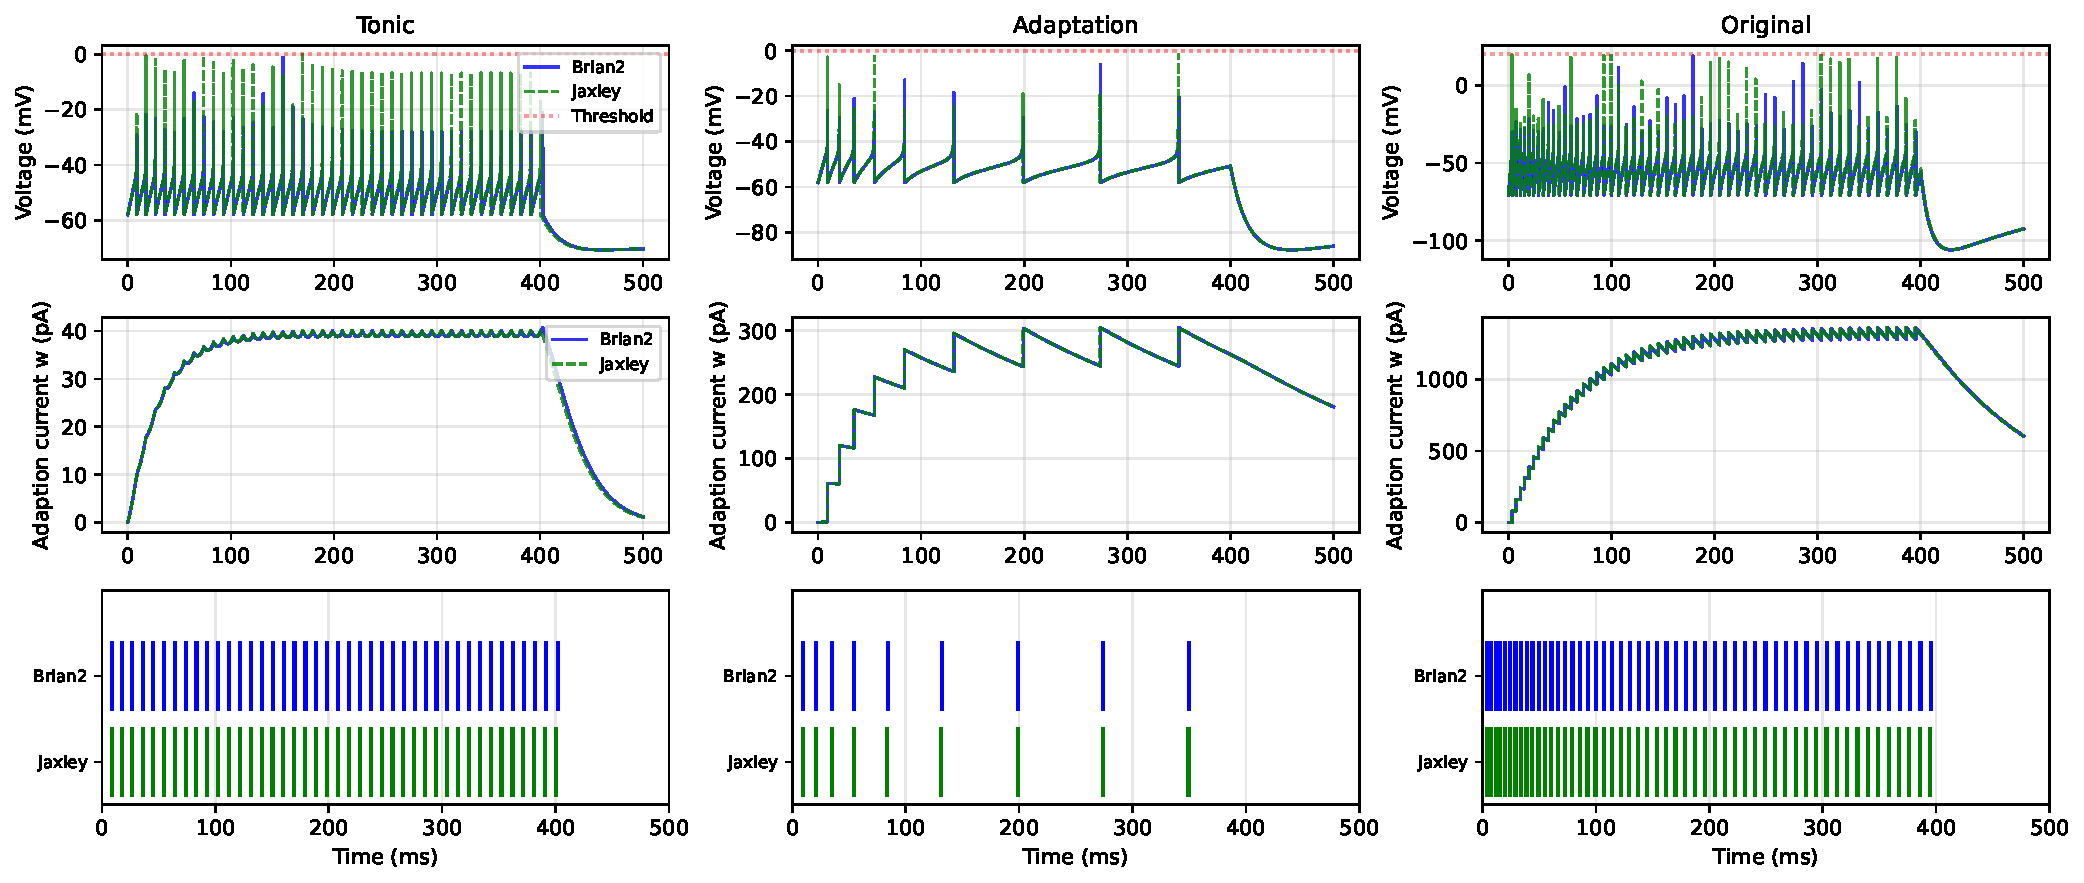
\includegraphics[width=\textwidth]{figures/adex_comparison_combined.pdf}
  \end{center}
  \caption{Left to right: tonic, adaption and original parameters.
Tonic and adaption parameters refer to the parameters provided by \cite{Naud2008}, original parameters are the parameters used in the original AdEx paper \cite{Brette2005}.
Top row shows the simulated voltage traces.
Interesting to note is that when the threshold is reached, the voltage is reset in the same time step.
This leads to the voltage never crossing the threshold line in the recordings.
Second row displays the adaption current $w$.
Last row compares the spike timings between \texttt{Brian2} and \texttt{Jaxley}.
We expect minor numerical differences, mainly to the fact that different integration methods are used.}\label{fig:brian_comparison}
\end{figure*}

To verify the correctness of our \gls{AdEx} implementation, we compare simulation outputs against Brian2 \cite{Stimberg2019}, a widely-used reference simulator for spiking neural networks.

\subsubsection{Comparison Setup}
Both simulators are configured identically:
\begin{itemize}
    \item Time step: $\Delta t = 0.01$ ms
    \item Simulation duration: 500 ms
    \item Stimulation duration: 400 ms
    \item Initial conditions: $V(0) = V_r$, $w(0) = 0$
\end{itemize}

\subsubsection{Test Cases}
We evaluate three parameter configurations from Naud et al.\ \cite{Naud2008} that produce distinct firing patterns:

\textbf{Tonic spiking}:\\
Regular spiking without spike-frequency adaptation, serving as a baseline case.
The parameters are the default parameters (see \ref{tab:adex_params}).

\textbf{Adaptation}:\\
Strong spike-triggered adaptation with slow decay, producing decreasing firing rates over time.
The parameters used are
$C_m = 200$,
$g_L = 12$,
$E_L = -70$,
$v_T = -50$,
$\Delta_T = 2$,
$v_r = -58$,
$v_{\text{threshold}} = 0$,
$\tau_w = 300$,
$a = 2$,
$b = 60$,
$I = 500$.

\textbf{Original parameters} \cite{Brette2005}:\\
The original parameter set from Brette and Gerstner, demonstrating combined adaptation mechanisms.
The parameters used are
$C_m = 281$,
$g_L = 30$,
$E_L = -70.6$,
$v_T = -50.4$,
$\Delta_T = 2$,
$v_r = -70.6$,
$v_{\text{threshold}} = 20$,
$\tau_w = 144$,
$a = 4$,
$b = 80.5$,
$I = 2500$.

\subsubsection{Comparison Metrics}\label{sec:comparison-metrics}
We assess implementation correctness through:
\begin{itemize}
  \item \textbf{Visual comparison:} Overlay of voltage traces from both simulators (Figure~\ref{fig:brian_comparison}).
  \item \textbf{Spike count:} Both implementations produce identical spike counts for all test configurations.
  \item \textbf{Spike timing:} Maximum absolute difference in spike times $\max_i |t_i^{\text{Jaxley}} - t_i^{\text{Brian2}}| < 1$ ms.
\end{itemize}

\section{Parameter Optimisation Evaluation}\label{sec:param_opt}
\ierror{Change this to Parameter Optimisation, make Evaluation it's own subsection}
\itodo{Introduce the testing framework to evaluate different loss functions, algorhithms, maybe hyperparamter optimization etc. etc.}

To evaluate the effectiveness of gradient-based optimisation with surrogate gradients, we fit \gls{AdEx} model parameters to experimental voltage recordings.
\begin{table}[thb]
\centering
\caption{Initial AdEx model parameters and trainability}
\label{tab:initial-params}
\begin{tabular}{lccc}
\toprule
\textbf{Parameter} & \textbf{Symbol} & \textbf{Initial Value} & \textbf{Trainable} \\
\midrule
Membrane capacitance & $C_m$ & 200.0\,pF & No \\
Leak conductance & $g_L$ & 10.0\,nS & Yes \\
Leak reversal potential & $E_L$ & $-68.0$\,mV & Yes \\
Spike threshold & $V_T$ & $-45.0$\,mV & Yes \\
Slope factor & $\Delta_T$ & 2.0\,mV & No \\
Spike detection threshold & $V_\text{threshold}$ & $-20.0$\,mV & No \\
Reset potential & $V_\text{reset}$ & $-55.0$\,mV & Yes \\
Adaptation time constant & $\tau_w$ & 100.0\,ms & Yes \\
Subthreshold adaptation & $a$ & 2.0\,nS & Yes \\
Spike-triggered adaptation & $b$ & 1.0\,pA & Yes \\
\bottomrule
\end{tabular}
\end{table}

\subsection{Dataset}\label{sec:data-set}
We use intracellular recordings from striatal projection neurons provided by Johansson and Silberberg \cite{Johansson2020}.
The dataset contains voltage traces from four distinct striatal neuron types, recorded under current-clamp conditions.
However, we only used a single trace\footnote{Files can be found \href{https://github.com/a1eko/humanspn/tree/df6ec55178c81e64fdcf4ae79aaa1872458c621f/models/optimisations/mCP-dspn-e150917_c6_D1-manimal_1_n24_04102017_cel1/expdata}{here}.
Voltage file: \texttt{ECBL\_IDthresh\_ch5\_553.dat}
Current file: \texttt{ECBL\_IDthresh\_ch4\_553.dat}}, mainly due to time constraint.
This is a serious limitation and will be addressed in future work.
\ierror{rewrite this!}

\subsection{Optimisation Setup}\label{sec:optimization-setup}
We optimise the following subset of \gls{AdEx} parameters: $\{g_L, E_L, V_T, a, b, \tau_w, v_{\text{reset}}\}$.
Parameters $\{C_m, \Delta_T, v_{\text{threshold}}$ were fixed.
Initial parameters are given in Table \ref{tab:initial-params}.

We evaluated two different loss functions: \gls{MSE} and a differentiable version of a feature based loss developed by Guarino et al.\cite{Guarino2025}, which we will name Guarino loss for the remaining report.
Detailed hyperparameters can be found in Table \ref{tab:training-params}, however, most parameters are chosen arbitrary.
No extensive hyperparameter tuning was conducted \mwarning{Maybe do this now? How extensive should I be? This should probably be it's own subsection}.
We plan on revising this in future work.

\begin{table}[t]
\centering
\caption{Training hyperparameters for AdEx optimization}
\label{tab:training-params}
\begin{tabular}{lcc}
\toprule
\textbf{Parameter} & \textbf{MSE} & \textbf{Guarino} \\
\midrule
\multicolumn{3}{l}{\textit{Optimization}} \\
Optimizer & Adam & Adam \\
Learning rate & 0.1 & 0.1 \\
Gradient clipping (global norm) & 2.0 & 2.0 \\
Number of epochs & 500 & 500 \\
\midrule
\multicolumn{3}{l}{\textit{Surrogate Gradient}} \\
Surrogate type & sigmoid & sigmoid \\
Surrogate slope & 25.0 & 25.0 \\
\midrule
\multicolumn{3}{l}{\textit{Loss-Specific Parameters}} \\
Normalize & False & --- \\
Temperature ($\tau$) & --- & 0.3 \\
Beta ($\beta$) & --- & 10.0 \\
Missing feature penalty & --- & 3.0 \\
\midrule
\multicolumn{3}{l}{\textit{Guarino Feature Weights}} \\
$w_{t_\text{first}}$ & --- & 5.0 \\
$w_{t_\text{second}}$ & --- & 3.0 \\
$w_{t_\text{third}}$ & --- & 2.0 \\
$w_{t_\text{last}}$ & --- & 1.0 \\
$w_{\text{inv\_first\_ISI}}$ & --- & 2.0 \\
$w_{\text{inv\_last\_ISI}}$ & --- & 1.0 \\
$w_{\text{firing\_freq}}$ & --- & 1.0 \\
$w_{V_\text{stim\_end}}$ & --- & 0.5 \\
\midrule
\multicolumn{3}{l}{\textit{Simulation}} \\
Max stimulus duration & \multicolumn{2}{c}{500\,ms} \\
Spike threshold & \multicolumn{2}{c}{$-20$\,mV} \\
\bottomrule
\end{tabular}
\end{table}

\subsection{Evaluation Metrics}\label{sec:evaluation-metrics}
We assess optimisation performance through:
\begin{itemize}
    \item Visual comparison of fitted vs.\ experimental traces
    \item Coincidence Factor for Spike Train Evaluation
    \item \itodo{wtime? runtime? iterations?}
    \item \itodo{Other qualatative metrics?}
\end{itemize}

The \textbf{Coincidence Factor for Spike Train Evaluation $\Gamma$} measures spike timing prediction quality, normalized by chance level.
It is given by
\begin{equation}
   \Gamma = \frac{N_{coinc} - \langle N_{coinc} \rangle}{0.5(N_{data} + N_{model})} \cdot \frac{1}{1 - 2f\Delta}
  \label{eq:coincidence-factor}
\end{equation}
where $N_{coinc}$ describe coincidences within $\pm\Delta$ (default 2ms)
and $f$ is the model firing rate.

In other words, it describes how good it compares to a random firing pattern. $\Gamma = 1$ means perfect prediction whereas $\Gamma = 0$ is the same as chance level.
$\Gamma < 0$ therefore means it behaves worse than chance.

Jolivet et al. achieved a $\Gamma$ value of $\approx 0.82-0.83$ for their well-fitted AdEx models.
We use this to compare our fitted parameters.
\ierror{Extend this with future work}

\section{Loss Functions}\label{sec:loss}

\mwarning{Could be Part of the Parameter optimization headline}

\subsection{MSE}\label{sec:mse-loss}
Our initial approach was to use \gls{MSE} as a loss function.
It is defined as
\begin{equation}\label{eq:MSE}
    \mathcal{L}_{\text{MSE}}(\theta) = \frac{1}{T} \sum_{t=1}^{T} \left( V_{\text{sim}}(t; \theta) - V_{\text{exp}}(t) \right)^2,
\end{equation}
where $\theta$ denotes the trainable parameters.

We were not able to achieve any sensible results using this loss function.
Since other works mainly use feature-based loss functions, we implemented one as well.

\subsection{Dynamic Time Warping}
\itodo{Implementation of dynamic time warping, then write this section}

\subsection{Feature-Based Loss}\label{sec:feature-loss}
Simplified neuron models are usually not required to perfectly imitate the voltage trace of a neuron.
Their main requirement is to faithfully replicate the firing behaviour.
Rather than comparing raw voltage traces, Guarino et al.~\cite{Guarino2025} proposed a loss function based on electrophysiological features:
To capture the essential characteristics of a neuron, they identified:
\begin{itemize}
    \item \textbf{Spike timing:} time to first ($t_1$), second ($t_2$), third ($t_3$), and last spike ($t_{\text{last}}$),
    \item \textbf{Interspike intervals:} inverse of first ISI ($\frac{1}{\text{ISI}_1}$) and last ISI ($\frac{1}{\text{ISI}_{\text{last}}}$),
    \item \textbf{Firing rate:} mean firing frequency over the stimulus duration,
    \item \textbf{Subthreshold behaviour:} membrane voltage at stimulus end ($V_{\text{stimend}}$).
\end{itemize}

The loss is computed as a weighted sum of relative errors:
\begin{equation}\label{eq:guarino}
    \mathcal{L}_{\text{Guarino}} = \sum_i w_i \cdot \frac{|f_i^{\text{sim}} - f_i^{\text{exp}}|}{|f_i^{\text{exp}}| + \epsilon}
\end{equation}
where $f_i^{\text{sim}}$ and $f_i^{\text{exp}}$ denote simulated and experimental feature values respectively, and $w_i$ are feature-specific weights.
When a feature is present in the experimental data but absent in the simulation (e.g., the experimental trace has three spikes but the simulation produces only one),
a fixed penalty is added to encourage the optimizer to produce the correct number of spikes.

This feature-based formulation addresses the spike timing sensitivity problem inherent to MSE:
small temporal misalignments no longer produce catastrophic loss values, as long as the overall firing pattern---captured by the features---remains similar.

\subsection{Differentiable Feature-Based Loss}\label{sec:diff-feature-loss}
The feature-based loss requires extracting spike times and counts from voltage traces.
Standard implementations use hard threshold crossings, which are non-differentiable.
To enable gradient-based optimization, we developed soft approximations of the feature extraction operations.

The core idea is to replace discrete spike detection with continuous values.
The AdExSurrogate channel outputs a soft spike indicator $s(t) \in [0, 1]$ at each time step.
The soft spike count becomes simply $N_{\text{spikes}}^{\text{soft}} = \sum_{t} s(t)$.

For spike timing, we use cumulative sums to identify when the $n$-th spike occurs and compute a weighted average over time.
Similarly, ISI features are derived from the difference between consecutive soft spike times.
Features that require a minimum number of spikes (e.g., ISI needs at least two spikes) are weighted by soft validity flags that smoothly transition based on the spike count.

The soft approximations introduce two hyperparameters: a temperature $\tau$ that controls how sharp the spike selection is, and a sigmoid steepness $\beta$ for the masking operations.
We used $\tau = 0.3$ and $\beta = 10.0$ based on initial experiments.

We note that this differentiable feature extraction is a working implementation that has not been thoroughly validated.
Due to time constraints, we did not perform extensive testing of the soft approximations against their hard counterparts, nor did we systematically tune the hyperparameters.
The approach produces gradients and enables optimization, but the accuracy of the soft features compared to exact values remains to be studied in future work.

\iwarning{I deleted the chapter for implementation. I think it's better suited as an integrated part of the methoodology. Be careful to be explicit and detailed on how things are implemeted!}

\section{Test Environment}\label{sec:testenv}
\itodo{Change section title}
\itodo{I can already write most of this because it will be my macbook for the most part anyway.}

\cleardoublepage
\chapter{Results}\label{ch:results}\deadline{May 15th}

\cleardoublepage
\chapter{Discussion}\label{ch:discussion}\deadline{May 31st}

\cleardoublepage
\chapter{Conclusions and Future work}\label{ch:conclusionsAndFutureWork}\deadline{May 31st}

\section{Conclusions}
\label{sec:conclusions}

\section{Limitations}
\label{sec:limitations}

\section{Future work}
\label{sec:futureWork}

\section{Reflections}
\label{sec:reflections}
\itodo{What are the relevant economic, social,
  environmental, and ethical aspects of your work?
}

\cleardoublepage
% Print the bibliography (and make it appear in the table of contents)
\printbibliography[heading=bibintoc]

% End of content
% ----------------------------------------------------------------------------------------------
% Appendix

\iwarning{If you do not have an appendix, do not include the \textbackslash cleardoublepage command below, otherwise the last page number in the meta data will be one too large.}
\cleardoublepage
\appendix
\renewcommand{\chaptermark}[1]{\markboth{Appendix \thechapter\relax:\thinspace\relax#1}{}}

\chapter{Appendix Chapter 1}
\section{Testing KTH colors}
\ifdigitaloutput
    \textbf{You have selected to optimize for digital output}
\else
    \textbf{You have selected to optimize for print output}
\fi
\begin{itemize}[noitemsep]
    \item Primary color
    \begin{itemize}
    \item \textcolor{kth-blue}{kth-blue \ifdigitaloutput
    actually Deep sea
    \fi} {\color{kth-blue} \rule{0.3\linewidth}{1mm} }\\

    \item \textcolor{kth-blue80}{kth-blue80} {\color{kth-blue80} \rule{0.3\linewidth}{1mm} }\\
\end{itemize}

\item  Secondary colors
\begin{itemize}[noitemsep]
    \item \textcolor{kth-lightblue}{kth-lightblue \ifdigitaloutput
    actually Stratosphere
    \fi} {\color{kth-lightblue} \rule{0.3\linewidth}{1mm} }\\

    \item \textcolor{kth-lightred}{kth-lightred \ifdigitaloutput
    actually Fluorescence\fi} {\color{kth-lightred} \rule{0.3\linewidth}{1mm} }\\

    \item \textcolor{kth-lightred80}{kth-lightred80} {\color{kth-lightred80} \rule{0.3\linewidth}{1mm} }\\

    \item \textcolor{kth-lightgreen}{kth-lightgreen \ifdigitaloutput
    actually Front-lawn\fi} {\color{kth-lightgreen} \rule{0.3\linewidth}{1mm} }\\

    \item \textcolor{kth-coolgray}{kth-coolgray \ifdigitaloutput
    actually Office\fi} {\color{kth-coolgray} \rule{0.3\linewidth}{1mm} }\\

    \item \textcolor{kth-coolgray80}{kth-coolgray80} {\color{kth-coolgray80} \rule{0.3\linewidth}{1mm} }
\end{itemize}
\end{itemize}

\textcolor{black}{black} {\color{black} \rule{\linewidth}{1mm} }


% End of Appendix
% ----------------------------------------------------------------------------------------------


%% The following label is necessary for computing the last page number of the body of the report to include in the "For DIVA" information
\label{pg:lastPageofMainmatter}

\cleardoublepage
\clearpage\thispagestyle{empty}\mbox{} % empty page with backcover on the other side
\kthbackcover
\fancyhead{}  % Do not use header on this extra page or pages
\section*{€€€€ For DIVA €€€€}
\lstset{numbers=none} %% remove any list line numbering
\divainfo{pg:lastPageofPreface}{pg:lastPageofMainmatter}

% If there is an acronyms.tex file,
% add it to the end of the For DIVA information
% so that it can be used with the abstracts
\IfFileExists{lib/acronyms.tex}{
\section*{acronyms.tex}
\lstinputlisting[language={[LaTeX]TeX}, basicstyle=\ttfamily\color{black},
commentstyle=\color{black}, backgroundcolor=\color{white}]{lib/acronyms.tex}
}
{}

\end{document}
